\documentclass{article}
\usepackage[utf8]{inputenc}
\usepackage[margin = 0.8in]{geometry}
\usepackage{graphicx}
\usepackage{amsmath, amssymb}
\usepackage{subcaption}
\usepackage{multirow}
\usepackage{mathtools}
\usepackage{float}


\title{RBE595 - Week 4 Assignment}
\author{Keith Chester}
\date{Due date: February 6, 2023}

\begin{document}
\maketitle

In this assignment, we prepared a simple gridworld with a robot that followed either a stochastic or a deterministic policy. In the deterministic polciy, we chose the highest possible score; if multiple tied this score, then an equal probability of selecting any of those higher scores. For the stochastic policy, we had an $80\%$ chance to select the highest value and a $20\%$ chance to select one of the adjacent directions within a 45 degree turn. If there were ties, then some combination of these tiles were selected per the probabilities dictated within the rules.

Here is a table that demonstrates the number of iterations and time it took to process each method of policy iteration, value iteration, and generalized policy iteration for both the deterministic and stochastic agents:

\begin{center}
    \begin{tabular}{ |cc|c|c| }
        \hline
        Method                       &               & Iterations & Seconds \\
        \hline
        Policy Iteration             &               &            &         \\
                                     & Deterministic & 31         & 5.21    \\
                                     & Stochastic    & 29         & 29.56   \\
        \hline
        Value Iteration              &               &            &         \\
                                     & Deterministic & 11         & 0.36    \\
                                     & Stochastic    & 10         & 0.45    \\
        \hline
        Generalized Policy Iteration &               &            &         \\
                                     & Deterministic & 20         & 0.65    \\
                                     & Stochastic    & 53         & 2.00    \\
        \hline
    \end{tabular}
\end{center}

\begin{figure}
    \begin{subfigure}{.5\textwidth}
        \centering
        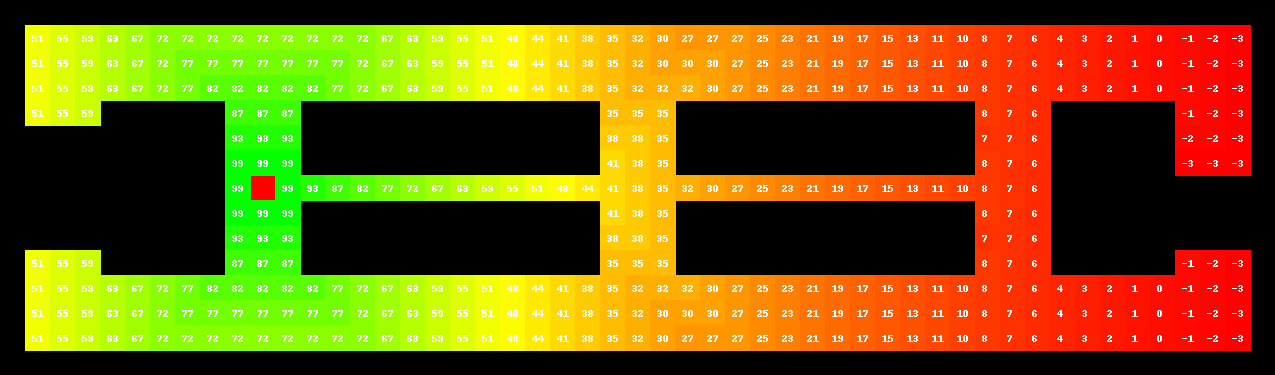
\includegraphics[width=.8\linewidth]{imgs/policy_iteration_value_map_deterministic.png}
        \caption{Deterministic Policy Iteration Value Map}
    \end{subfigure}
    \begin{subfigure}{.5\textwidth}
        \centering
        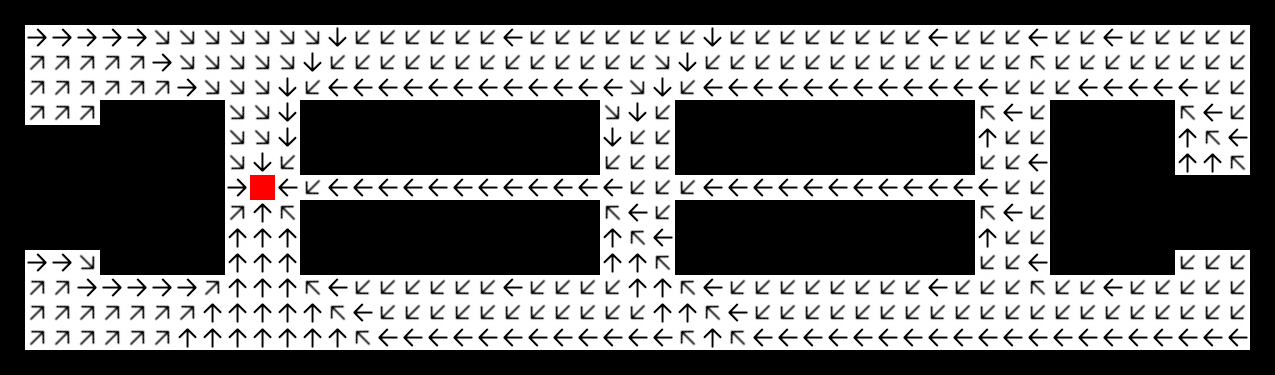
\includegraphics[width=.8\linewidth]{imgs/polciy_iteration_policy_map_deterministic.png}
        \caption{Deterministic Policy Iteration Policy Map}
    \end{subfigure}
    \begin{subfigure}{.5\textwidth}
        \centering
        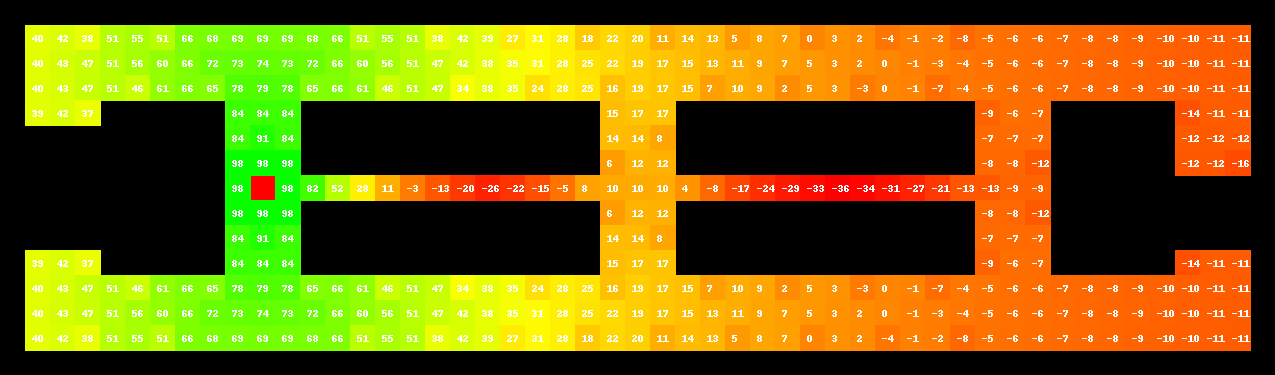
\includegraphics[width=.8\linewidth]{imgs/policy_iteration_value_map_stochastic.png}
        \caption{Stochastic Policy Iteration Value Map}
    \end{subfigure}
    \begin{subfigure}{.5\textwidth}
        \centering
        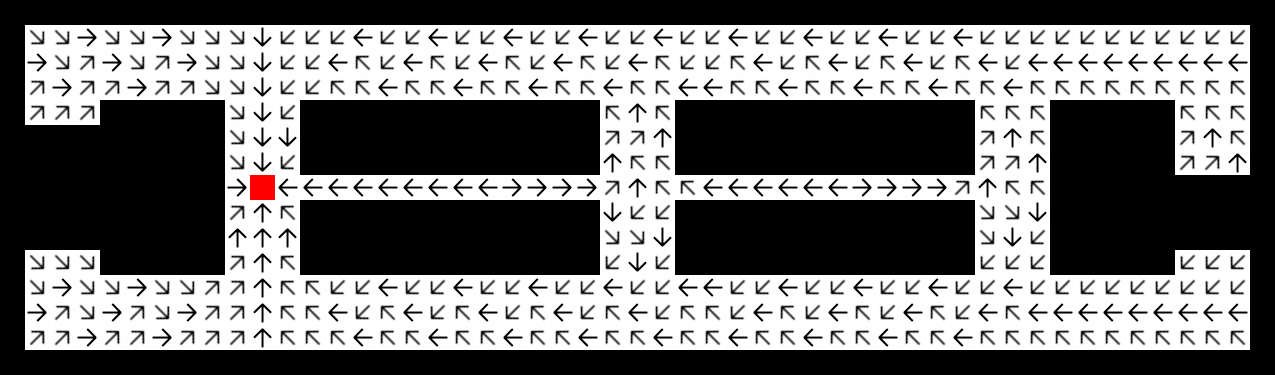
\includegraphics[width=.8\linewidth]{imgs/polciy_iteration_policy_map_stochastic.png}
        \caption{Stochastic Policy Iteration Value Map}
    \end{subfigure}
    \caption{Policy and value maps generated with Policy Iteration}
\end{figure}

\begin{figure}
    \begin{subfigure}{.5\textwidth}
        \centering
        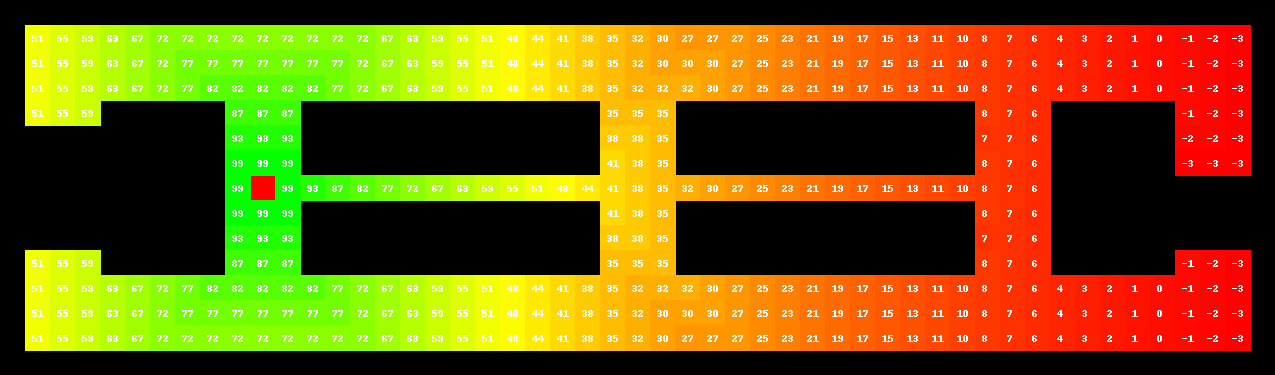
\includegraphics[width=.8\linewidth]{imgs/value_iteration_value_map_deterministic.png}
        \caption{Deterministic Value Iteration Value Map}
    \end{subfigure}
    \begin{subfigure}{.5\textwidth}
        \centering
        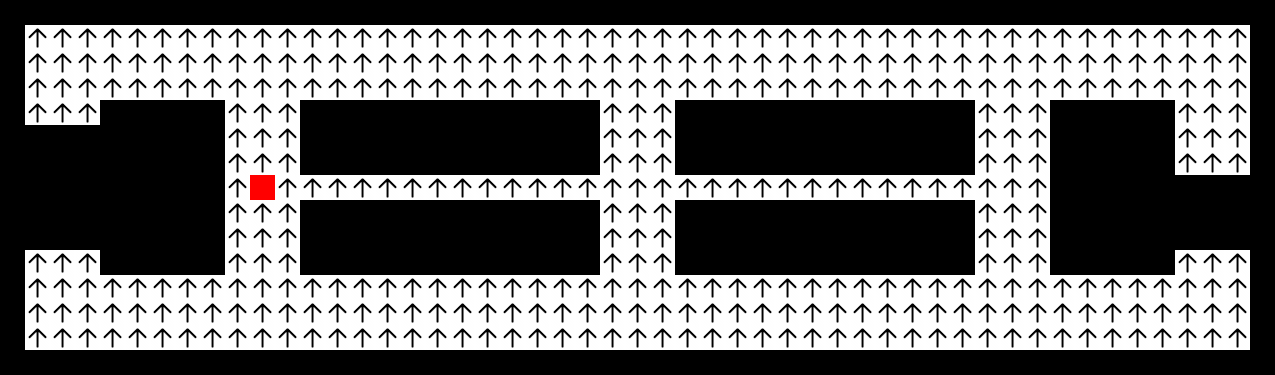
\includegraphics[width=.8\linewidth]{imgs/value_iteration_policy_map_deterministic.png}
        \caption{Deterministic Value Iteration Policy Map}
    \end{subfigure}
    \begin{subfigure}{.5\textwidth}
        \centering
        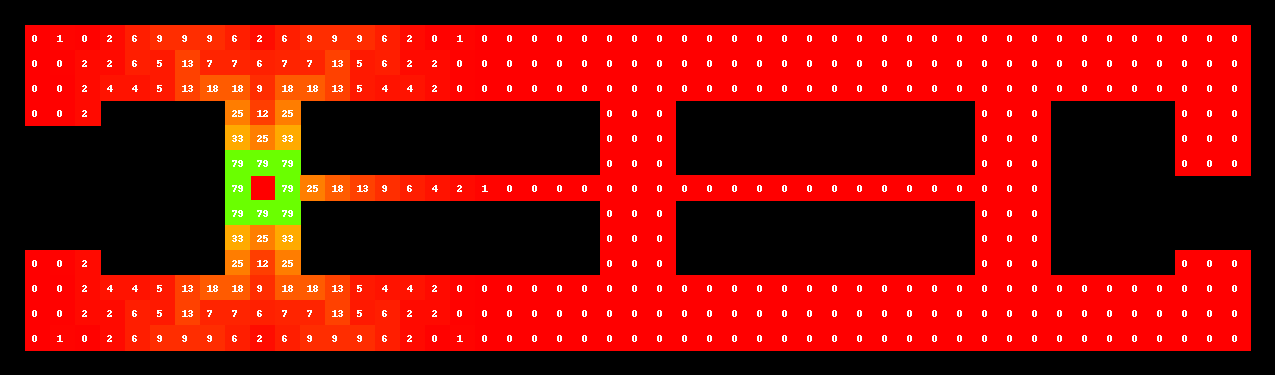
\includegraphics[width=.8\linewidth]{imgs/value_iteration_value_map_stochastic.png}
        \caption{Stochastic Value Iteration Value Map}
    \end{subfigure}
    \begin{subfigure}{.5\textwidth}
        \centering
        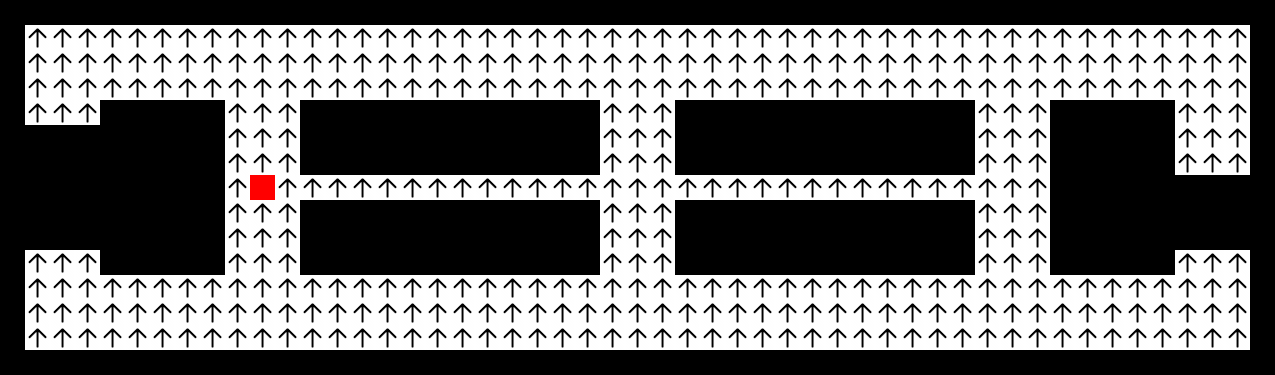
\includegraphics[width=.8\linewidth]{imgs/value_iteration_policy_map_stochastic.png}
        \caption{Stochastic Value Iteration Value Map}
    \end{subfigure}
    \caption{Policy and value maps generated with Value Iteration}
\end{figure}

\begin{figure}
    \begin{subfigure}{.5\textwidth}
        \centering
        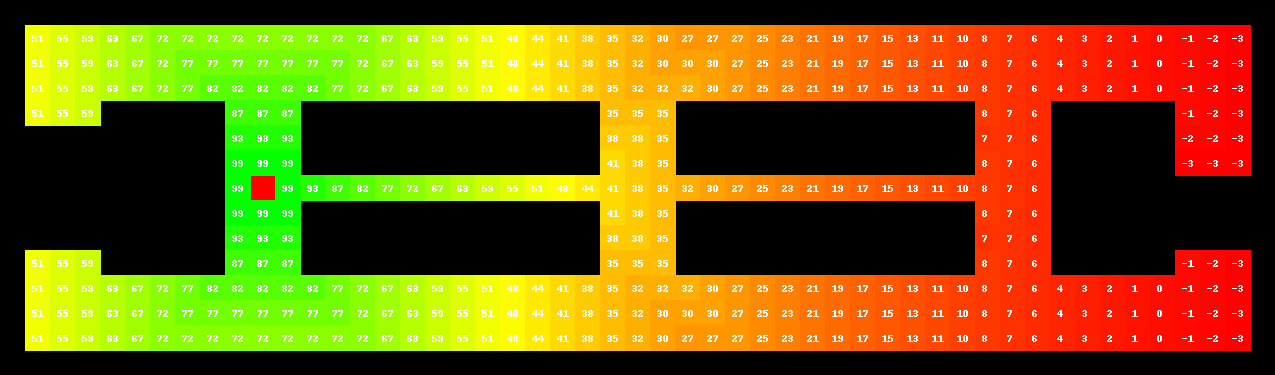
\includegraphics[width=.8\linewidth]{imgs/generalized_policy_iteration_value_map_deterministic.png}
        \caption{Deterministic Generalized Policy Iteration Value Map}
    \end{subfigure}
    \begin{subfigure}{.5\textwidth}
        \centering
        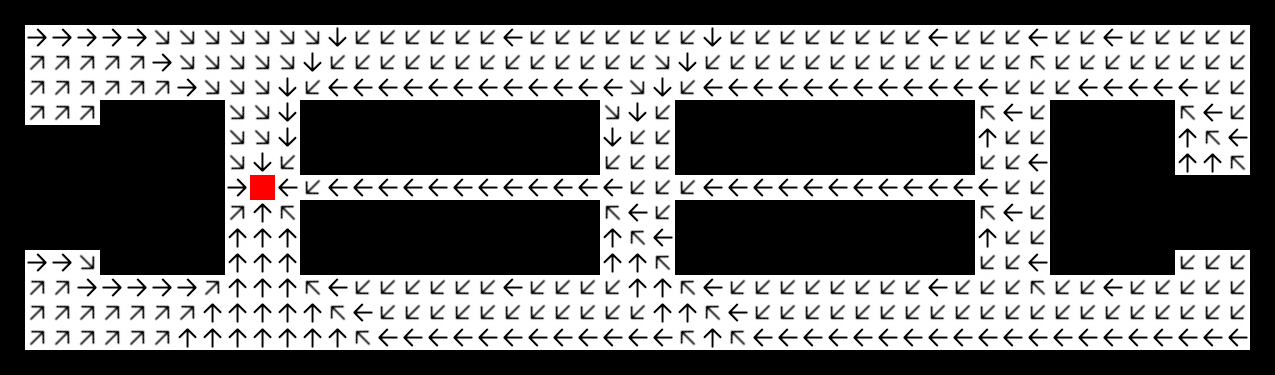
\includegraphics[width=.8\linewidth]{imgs/generalized_policy_iteration_policy_map_deterministic.png}
        \caption{Deterministic Generalized Policy Iteration Policy Map}
    \end{subfigure}
    \begin{subfigure}{.5\textwidth}
        \centering
        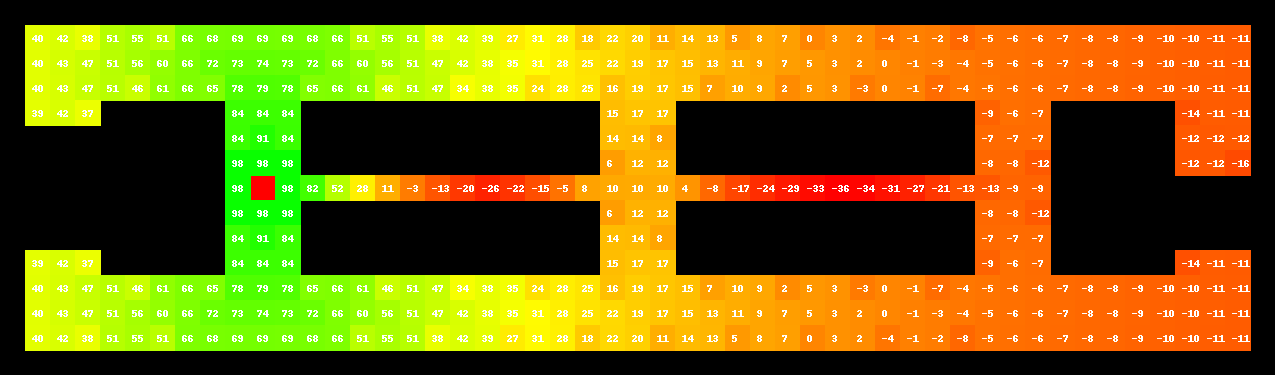
\includegraphics[width=.8\linewidth]{imgs/generalized_policy_iteration_value_map_stochastic.png}
        \caption{Stochastic Generalized Policy Iteration Value Map}
    \end{subfigure}
    \begin{subfigure}{.5\textwidth}
        \centering
        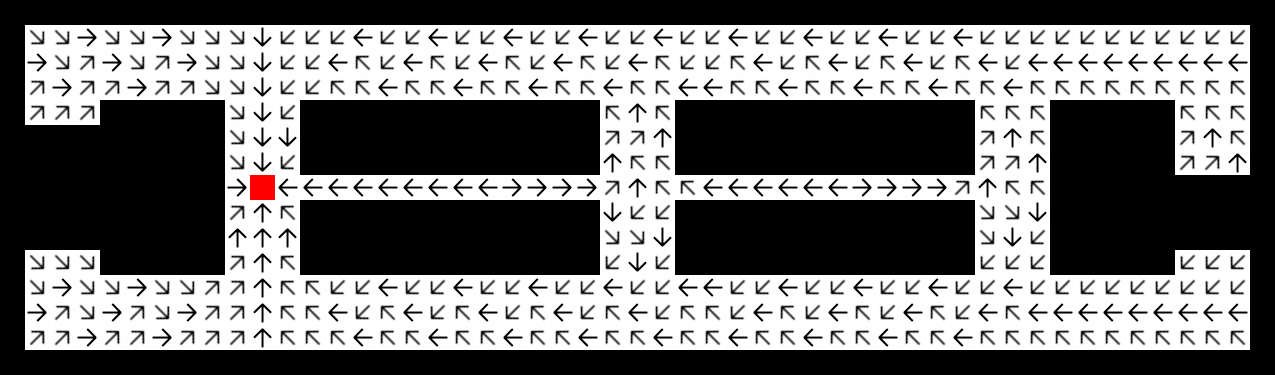
\includegraphics[width=.8\linewidth]{imgs/generalized_policy_iteration_policy_map_stochastic.png}
        \caption{Stochastic Generalized Policy Iteration Value Map}
    \end{subfigure}
    \caption{Policy and value maps generated with Generalized Policy Iteration}
\end{figure}



\end{document}